\documentclass[twoside]{book}

% Packages required by doxygen
\usepackage{calc}
\usepackage{doxygen}
\usepackage{graphicx}
\usepackage[utf8]{inputenc}
\usepackage{makeidx}
\usepackage{multicol}
\usepackage{multirow}
\usepackage{textcomp}
\usepackage[table]{xcolor}

% Font selection
\usepackage[T1]{fontenc}
\usepackage{mathptmx}
\usepackage[scaled=.90]{helvet}
\usepackage{courier}
\usepackage{amssymb}
\usepackage{sectsty}
\renewcommand{\familydefault}{\sfdefault}
\allsectionsfont{%
  \fontseries{bc}\selectfont%
  \color{darkgray}%
}
\renewcommand{\DoxyLabelFont}{%
  \fontseries{bc}\selectfont%
  \color{darkgray}%
}

% Page & text layout
\usepackage{geometry}
\geometry{%
  a4paper,%
  top=2.5cm,%
  bottom=2.5cm,%
  left=2.5cm,%
  right=2.5cm%
}
\tolerance=750
\hfuzz=15pt
\hbadness=750
\setlength{\emergencystretch}{15pt}
\setlength{\parindent}{0cm}
\setlength{\parskip}{0.2cm}
\makeatletter
\renewcommand{\paragraph}{%
  \@startsection{paragraph}{4}{0ex}{-1.0ex}{1.0ex}{%
    \normalfont\normalsize\bfseries\SS@parafont%
  }%
}
\renewcommand{\subparagraph}{%
  \@startsection{subparagraph}{5}{0ex}{-1.0ex}{1.0ex}{%
    \normalfont\normalsize\bfseries\SS@subparafont%
  }%
}
\makeatother

% Headers & footers
\usepackage{fancyhdr}
\pagestyle{fancyplain}
\fancyhead[LE]{\fancyplain{}{\bfseries\thepage}}
\fancyhead[CE]{\fancyplain{}{}}
\fancyhead[RE]{\fancyplain{}{\bfseries\leftmark}}
\fancyhead[LO]{\fancyplain{}{\bfseries\rightmark}}
\fancyhead[CO]{\fancyplain{}{}}
\fancyhead[RO]{\fancyplain{}{\bfseries\thepage}}
\fancyfoot[LE]{\fancyplain{}{}}
\fancyfoot[CE]{\fancyplain{}{}}
\fancyfoot[RE]{\fancyplain{}{\bfseries\scriptsize Generated on Tue Sep 13 2016 11\-:12\-:34 for Probabilistic Star\-Vars by Doxygen }}
\fancyfoot[LO]{\fancyplain{}{\bfseries\scriptsize Generated on Tue Sep 13 2016 11\-:12\-:34 for Probabilistic Star\-Vars by Doxygen }}
\fancyfoot[CO]{\fancyplain{}{}}
\fancyfoot[RO]{\fancyplain{}{}}
\renewcommand{\footrulewidth}{0.4pt}
\renewcommand{\chaptermark}[1]{%
  \markboth{#1}{}%
}
\renewcommand{\sectionmark}[1]{%
  \markright{\thesection\ #1}%
}

% Indices & bibliography
\usepackage{natbib}
\usepackage[titles]{tocloft}
\setcounter{tocdepth}{3}
\setcounter{secnumdepth}{5}
\makeindex

% Hyperlinks (required, but should be loaded last)
\usepackage{ifpdf}
\ifpdf
  \usepackage[pdftex,pagebackref=true]{hyperref}
\else
  \usepackage[ps2pdf,pagebackref=true]{hyperref}
\fi
\hypersetup{%
  colorlinks=true,%
  linkcolor=blue,%
  citecolor=blue,%
  unicode%
}

% Custom commands
\newcommand{\clearemptydoublepage}{%
  \newpage{\pagestyle{empty}\cleardoublepage}%
}


%===== C O N T E N T S =====

\begin{document}

% Titlepage & ToC
\hypersetup{pageanchor=false}
\pagenumbering{roman}
\begin{titlepage}
\vspace*{7cm}
\begin{center}%
{\Large Probabilistic Star\-Vars }\\
\vspace*{1cm}
{\large Generated by Doxygen 1.8.6}\\
\vspace*{0.5cm}
{\small Tue Sep 13 2016 11:12:34}\\
\end{center}
\end{titlepage}
\clearemptydoublepage
\tableofcontents
\clearemptydoublepage
\pagenumbering{arabic}
\hypersetup{pageanchor=true}

%--- Begin generated contents ---
\chapter{Namespace Index}
\section{Namespace List}
Here is a list of all namespaces with brief descriptions\-:\begin{DoxyCompactList}
\item\contentsline{section}{\hyperlink{namespacemain}{main} }{\pageref{namespacemain}}{}
\item\contentsline{section}{\hyperlink{namespaceoriented__point}{oriented\-\_\-point} }{\pageref{namespaceoriented__point}}{}
\item\contentsline{section}{\hyperlink{namespacestarvars}{starvars} }{\pageref{namespacestarvars}}{}
\end{DoxyCompactList}

\chapter{Class Index}
\section{Class List}
Here are the classes, structs, unions and interfaces with brief descriptions\-:\begin{DoxyCompactList}
\item\contentsline{section}{\hyperlink{classoriented__point_1_1OrientedPoint}{oriented\-\_\-point.\-Oriented\-Point} }{\pageref{classoriented__point_1_1OrientedPoint}}{}
\item\contentsline{section}{\hyperlink{classstarvars_1_1StarVars}{starvars.\-Star\-Vars} }{\pageref{classstarvars_1_1StarVars}}{}
\end{DoxyCompactList}

\chapter{File Index}
\section{File List}
Here is a list of all files with brief descriptions\-:\begin{DoxyCompactList}
\item\contentsline{section}{\hyperlink{main_8py}{main.\-py} }{\pageref{main_8py}}{}
\item\contentsline{section}{\hyperlink{oriented__point_8py}{oriented\-\_\-point.\-py} }{\pageref{oriented__point_8py}}{}
\item\contentsline{section}{\hyperlink{starvars_8py}{starvars.\-py} }{\pageref{starvars_8py}}{}
\end{DoxyCompactList}

\chapter{Namespace Documentation}
\hypertarget{namespacemain}{\section{main Namespace Reference}
\label{namespacemain}\index{main@{main}}
}
\subsection*{Functions}
\begin{DoxyCompactItemize}
\item 
def \hyperlink{namespacemain_a021bfca46dd0435fb213d09cf10db27e}{main}
\end{DoxyCompactItemize}
\subsection*{Variables}
\begin{DoxyCompactItemize}
\item 
string \hyperlink{namespacemain_a5e2661c5c42dc197ee8e68887453d3bc}{\-\_\-\-\_\-author\-\_\-\-\_\-} = \char`\"{}Danilo H. Perico\char`\"{}
\item 
string \hyperlink{namespacemain_a70420639202607ff61f0a08061e04e47}{\-\_\-\-\_\-license\-\_\-\-\_\-} = \char`\"{}G\-N\-U General Public License v3.\-0\char`\"{}
\item 
string \hyperlink{namespacemain_afb7b6dcaed6631460aa4089c3b178748}{\-\_\-\-\_\-project\-\_\-\-\_\-} = \char`\"{}Probabilistic \hyperlink{classstarvars_1_1StarVars}{Star\-Vars}\char`\"{}
\end{DoxyCompactItemize}


\subsection{Function Documentation}
\hypertarget{namespacemain_a021bfca46dd0435fb213d09cf10db27e}{\index{main@{main}!main@{main}}
\index{main@{main}!main@{main}}
\subsubsection[{main}]{\setlength{\rightskip}{0pt plus 5cm}def main.\-main (
\begin{DoxyParamCaption}
{}
\end{DoxyParamCaption}
)}}\label{namespacemain_a021bfca46dd0435fb213d09cf10db27e}


\subsection{Variable Documentation}
\hypertarget{namespacemain_a5e2661c5c42dc197ee8e68887453d3bc}{\index{main@{main}!\-\_\-\-\_\-author\-\_\-\-\_\-@{\-\_\-\-\_\-author\-\_\-\-\_\-}}
\index{\-\_\-\-\_\-author\-\_\-\-\_\-@{\-\_\-\-\_\-author\-\_\-\-\_\-}!main@{main}}
\subsubsection[{\-\_\-\-\_\-author\-\_\-\-\_\-}]{\setlength{\rightskip}{0pt plus 5cm}string main.\-\_\-\-\_\-author\-\_\-\-\_\- = \char`\"{}Danilo H. Perico\char`\"{}}}\label{namespacemain_a5e2661c5c42dc197ee8e68887453d3bc}
\hypertarget{namespacemain_a70420639202607ff61f0a08061e04e47}{\index{main@{main}!\-\_\-\-\_\-license\-\_\-\-\_\-@{\-\_\-\-\_\-license\-\_\-\-\_\-}}
\index{\-\_\-\-\_\-license\-\_\-\-\_\-@{\-\_\-\-\_\-license\-\_\-\-\_\-}!main@{main}}
\subsubsection[{\-\_\-\-\_\-license\-\_\-\-\_\-}]{\setlength{\rightskip}{0pt plus 5cm}string main.\-\_\-\-\_\-license\-\_\-\-\_\- = \char`\"{}G\-N\-U General Public License v3.\-0\char`\"{}}}\label{namespacemain_a70420639202607ff61f0a08061e04e47}
\hypertarget{namespacemain_afb7b6dcaed6631460aa4089c3b178748}{\index{main@{main}!\-\_\-\-\_\-project\-\_\-\-\_\-@{\-\_\-\-\_\-project\-\_\-\-\_\-}}
\index{\-\_\-\-\_\-project\-\_\-\-\_\-@{\-\_\-\-\_\-project\-\_\-\-\_\-}!main@{main}}
\subsubsection[{\-\_\-\-\_\-project\-\_\-\-\_\-}]{\setlength{\rightskip}{0pt plus 5cm}string main.\-\_\-\-\_\-project\-\_\-\-\_\- = \char`\"{}Probabilistic {\bf Star\-Vars}\char`\"{}}}\label{namespacemain_afb7b6dcaed6631460aa4089c3b178748}

\hypertarget{namespaceoriented__point}{\section{oriented\-\_\-point Namespace Reference}
\label{namespaceoriented__point}\index{oriented\-\_\-point@{oriented\-\_\-point}}
}
\subsection*{Classes}
\begin{DoxyCompactItemize}
\item 
class \hyperlink{classoriented__point_1_1OrientedPoint}{Oriented\-Point}
\end{DoxyCompactItemize}
\subsection*{Variables}
\begin{DoxyCompactItemize}
\item 
string \hyperlink{namespaceoriented__point_aa3b4d2d674d85c3cbe62dd838254d6d0}{\-\_\-\-\_\-author\-\_\-\-\_\-} = \char`\"{}Danilo H. Perico\char`\"{}
\item 
string \hyperlink{namespaceoriented__point_a3d6cc46d63eaa6bbf92eff2835e6a1c2}{\-\_\-\-\_\-license\-\_\-\-\_\-} = \char`\"{}G\-N\-U General Public License v3.\-0\char`\"{}
\item 
string \hyperlink{namespaceoriented__point_a9691eace975baee6e55c7185dc3bb251}{\-\_\-\-\_\-project\-\_\-\-\_\-} = \char`\"{}Probabilistic Star\-Vars\char`\"{}
\end{DoxyCompactItemize}


\subsection{Variable Documentation}
\hypertarget{namespaceoriented__point_aa3b4d2d674d85c3cbe62dd838254d6d0}{\index{oriented\-\_\-point@{oriented\-\_\-point}!\-\_\-\-\_\-author\-\_\-\-\_\-@{\-\_\-\-\_\-author\-\_\-\-\_\-}}
\index{\-\_\-\-\_\-author\-\_\-\-\_\-@{\-\_\-\-\_\-author\-\_\-\-\_\-}!oriented_point@{oriented\-\_\-point}}
\subsubsection[{\-\_\-\-\_\-author\-\_\-\-\_\-}]{\setlength{\rightskip}{0pt plus 5cm}string oriented\-\_\-point.\-\_\-\-\_\-author\-\_\-\-\_\- = \char`\"{}Danilo H. Perico\char`\"{}}}\label{namespaceoriented__point_aa3b4d2d674d85c3cbe62dd838254d6d0}
\hypertarget{namespaceoriented__point_a3d6cc46d63eaa6bbf92eff2835e6a1c2}{\index{oriented\-\_\-point@{oriented\-\_\-point}!\-\_\-\-\_\-license\-\_\-\-\_\-@{\-\_\-\-\_\-license\-\_\-\-\_\-}}
\index{\-\_\-\-\_\-license\-\_\-\-\_\-@{\-\_\-\-\_\-license\-\_\-\-\_\-}!oriented_point@{oriented\-\_\-point}}
\subsubsection[{\-\_\-\-\_\-license\-\_\-\-\_\-}]{\setlength{\rightskip}{0pt plus 5cm}string oriented\-\_\-point.\-\_\-\-\_\-license\-\_\-\-\_\- = \char`\"{}G\-N\-U General Public License v3.\-0\char`\"{}}}\label{namespaceoriented__point_a3d6cc46d63eaa6bbf92eff2835e6a1c2}
\hypertarget{namespaceoriented__point_a9691eace975baee6e55c7185dc3bb251}{\index{oriented\-\_\-point@{oriented\-\_\-point}!\-\_\-\-\_\-project\-\_\-\-\_\-@{\-\_\-\-\_\-project\-\_\-\-\_\-}}
\index{\-\_\-\-\_\-project\-\_\-\-\_\-@{\-\_\-\-\_\-project\-\_\-\-\_\-}!oriented_point@{oriented\-\_\-point}}
\subsubsection[{\-\_\-\-\_\-project\-\_\-\-\_\-}]{\setlength{\rightskip}{0pt plus 5cm}string oriented\-\_\-point.\-\_\-\-\_\-project\-\_\-\-\_\- = \char`\"{}Probabilistic Star\-Vars\char`\"{}}}\label{namespaceoriented__point_a9691eace975baee6e55c7185dc3bb251}

\hypertarget{namespacestarvars}{\section{starvars Namespace Reference}
\label{namespacestarvars}\index{starvars@{starvars}}
}
\subsection*{Classes}
\begin{DoxyCompactItemize}
\item 
class \hyperlink{classstarvars_1_1StarVars}{Star\-Vars}
\end{DoxyCompactItemize}
\subsection*{Variables}
\begin{DoxyCompactItemize}
\item 
string \hyperlink{namespacestarvars_ac644d7f280f95cccc18a5d57a812e131}{\-\_\-\-\_\-author\-\_\-\-\_\-} = \char`\"{}Danilo H. Perico\char`\"{}
\item 
string \hyperlink{namespacestarvars_a1264921cafa3bfaea6a08a307416bbc6}{\-\_\-\-\_\-license\-\_\-\-\_\-} = \char`\"{}G\-N\-U General Public License v3.\-0\char`\"{}
\item 
string \hyperlink{namespacestarvars_afabb4c7baf270d344e2640778b38e5ff}{\-\_\-\-\_\-project\-\_\-\-\_\-} = \char`\"{}Probabilistic \hyperlink{classstarvars_1_1StarVars}{Star\-Vars}\char`\"{}
\end{DoxyCompactItemize}


\subsection{Variable Documentation}
\hypertarget{namespacestarvars_ac644d7f280f95cccc18a5d57a812e131}{\index{starvars@{starvars}!\-\_\-\-\_\-author\-\_\-\-\_\-@{\-\_\-\-\_\-author\-\_\-\-\_\-}}
\index{\-\_\-\-\_\-author\-\_\-\-\_\-@{\-\_\-\-\_\-author\-\_\-\-\_\-}!starvars@{starvars}}
\subsubsection[{\-\_\-\-\_\-author\-\_\-\-\_\-}]{\setlength{\rightskip}{0pt plus 5cm}string starvars.\-\_\-\-\_\-author\-\_\-\-\_\- = \char`\"{}Danilo H. Perico\char`\"{}}}\label{namespacestarvars_ac644d7f280f95cccc18a5d57a812e131}
\hypertarget{namespacestarvars_a1264921cafa3bfaea6a08a307416bbc6}{\index{starvars@{starvars}!\-\_\-\-\_\-license\-\_\-\-\_\-@{\-\_\-\-\_\-license\-\_\-\-\_\-}}
\index{\-\_\-\-\_\-license\-\_\-\-\_\-@{\-\_\-\-\_\-license\-\_\-\-\_\-}!starvars@{starvars}}
\subsubsection[{\-\_\-\-\_\-license\-\_\-\-\_\-}]{\setlength{\rightskip}{0pt plus 5cm}string starvars.\-\_\-\-\_\-license\-\_\-\-\_\- = \char`\"{}G\-N\-U General Public License v3.\-0\char`\"{}}}\label{namespacestarvars_a1264921cafa3bfaea6a08a307416bbc6}
\hypertarget{namespacestarvars_afabb4c7baf270d344e2640778b38e5ff}{\index{starvars@{starvars}!\-\_\-\-\_\-project\-\_\-\-\_\-@{\-\_\-\-\_\-project\-\_\-\-\_\-}}
\index{\-\_\-\-\_\-project\-\_\-\-\_\-@{\-\_\-\-\_\-project\-\_\-\-\_\-}!starvars@{starvars}}
\subsubsection[{\-\_\-\-\_\-project\-\_\-\-\_\-}]{\setlength{\rightskip}{0pt plus 5cm}string starvars.\-\_\-\-\_\-project\-\_\-\-\_\- = \char`\"{}Probabilistic {\bf Star\-Vars}\char`\"{}}}\label{namespacestarvars_afabb4c7baf270d344e2640778b38e5ff}

\chapter{Class Documentation}
\hypertarget{classoriented__point_1_1OrientedPoint}{\section{oriented\-\_\-point.\-Oriented\-Point Class Reference}
\label{classoriented__point_1_1OrientedPoint}\index{oriented\-\_\-point.\-Oriented\-Point@{oriented\-\_\-point.\-Oriented\-Point}}
}


Collaboration diagram for oriented\-\_\-point.\-Oriented\-Point\-:\nopagebreak
\begin{figure}[H]
\begin{center}
\leavevmode
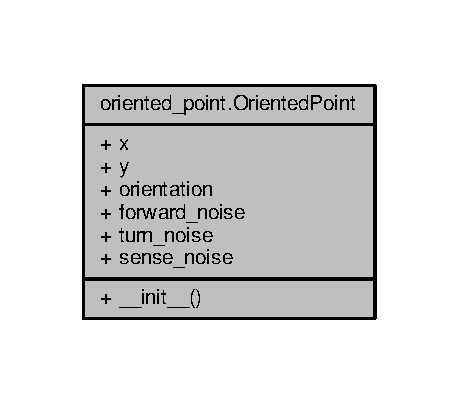
\includegraphics[width=220pt]{classoriented__point_1_1OrientedPoint__coll__graph}
\end{center}
\end{figure}
\subsection*{Public Member Functions}
\begin{DoxyCompactItemize}
\item 
def \hyperlink{classoriented__point_1_1OrientedPoint_a01289ef0dcb80af4b61c4c8352c82639}{\-\_\-\-\_\-init\-\_\-\-\_\-}
\end{DoxyCompactItemize}
\subsection*{Public Attributes}
\begin{DoxyCompactItemize}
\item 
\hyperlink{classoriented__point_1_1OrientedPoint_a020fc32ac0c377591b1d7686c66310ac}{x}
\item 
\hyperlink{classoriented__point_1_1OrientedPoint_a9f9f32b6143828eefe2c768680b9ac44}{y}
\item 
\hyperlink{classoriented__point_1_1OrientedPoint_a7a95e72e5f5ac1de5d3c1314c19a8c5d}{orientation}
\item 
\hyperlink{classoriented__point_1_1OrientedPoint_a5e69ec880e4e02b4c6cbf7b7b528eaf0}{forward\-\_\-noise}
\item 
\hyperlink{classoriented__point_1_1OrientedPoint_a2f90057368b176f551cf9c94166724bd}{turn\-\_\-noise}
\item 
\hyperlink{classoriented__point_1_1OrientedPoint_a6a5ce78d8ea5234a60920f7e0e3c485d}{sense\-\_\-noise}
\end{DoxyCompactItemize}


\subsection{Constructor \& Destructor Documentation}
\hypertarget{classoriented__point_1_1OrientedPoint_a01289ef0dcb80af4b61c4c8352c82639}{\index{oriented\-\_\-point\-::\-Oriented\-Point@{oriented\-\_\-point\-::\-Oriented\-Point}!\-\_\-\-\_\-init\-\_\-\-\_\-@{\-\_\-\-\_\-init\-\_\-\-\_\-}}
\index{\-\_\-\-\_\-init\-\_\-\-\_\-@{\-\_\-\-\_\-init\-\_\-\-\_\-}!oriented_point::OrientedPoint@{oriented\-\_\-point\-::\-Oriented\-Point}}
\subsubsection[{\-\_\-\-\_\-init\-\_\-\-\_\-}]{\setlength{\rightskip}{0pt plus 5cm}def oriented\-\_\-point.\-Oriented\-Point.\-\_\-\-\_\-init\-\_\-\-\_\- (
\begin{DoxyParamCaption}
\item[{}]{self}
\end{DoxyParamCaption}
)}}\label{classoriented__point_1_1OrientedPoint_a01289ef0dcb80af4b61c4c8352c82639}


\subsection{Member Data Documentation}
\hypertarget{classoriented__point_1_1OrientedPoint_a5e69ec880e4e02b4c6cbf7b7b528eaf0}{\index{oriented\-\_\-point\-::\-Oriented\-Point@{oriented\-\_\-point\-::\-Oriented\-Point}!forward\-\_\-noise@{forward\-\_\-noise}}
\index{forward\-\_\-noise@{forward\-\_\-noise}!oriented_point::OrientedPoint@{oriented\-\_\-point\-::\-Oriented\-Point}}
\subsubsection[{forward\-\_\-noise}]{\setlength{\rightskip}{0pt plus 5cm}oriented\-\_\-point.\-Oriented\-Point.\-forward\-\_\-noise}}\label{classoriented__point_1_1OrientedPoint_a5e69ec880e4e02b4c6cbf7b7b528eaf0}
\hypertarget{classoriented__point_1_1OrientedPoint_a7a95e72e5f5ac1de5d3c1314c19a8c5d}{\index{oriented\-\_\-point\-::\-Oriented\-Point@{oriented\-\_\-point\-::\-Oriented\-Point}!orientation@{orientation}}
\index{orientation@{orientation}!oriented_point::OrientedPoint@{oriented\-\_\-point\-::\-Oriented\-Point}}
\subsubsection[{orientation}]{\setlength{\rightskip}{0pt plus 5cm}oriented\-\_\-point.\-Oriented\-Point.\-orientation}}\label{classoriented__point_1_1OrientedPoint_a7a95e72e5f5ac1de5d3c1314c19a8c5d}
\hypertarget{classoriented__point_1_1OrientedPoint_a6a5ce78d8ea5234a60920f7e0e3c485d}{\index{oriented\-\_\-point\-::\-Oriented\-Point@{oriented\-\_\-point\-::\-Oriented\-Point}!sense\-\_\-noise@{sense\-\_\-noise}}
\index{sense\-\_\-noise@{sense\-\_\-noise}!oriented_point::OrientedPoint@{oriented\-\_\-point\-::\-Oriented\-Point}}
\subsubsection[{sense\-\_\-noise}]{\setlength{\rightskip}{0pt plus 5cm}oriented\-\_\-point.\-Oriented\-Point.\-sense\-\_\-noise}}\label{classoriented__point_1_1OrientedPoint_a6a5ce78d8ea5234a60920f7e0e3c485d}
\hypertarget{classoriented__point_1_1OrientedPoint_a2f90057368b176f551cf9c94166724bd}{\index{oriented\-\_\-point\-::\-Oriented\-Point@{oriented\-\_\-point\-::\-Oriented\-Point}!turn\-\_\-noise@{turn\-\_\-noise}}
\index{turn\-\_\-noise@{turn\-\_\-noise}!oriented_point::OrientedPoint@{oriented\-\_\-point\-::\-Oriented\-Point}}
\subsubsection[{turn\-\_\-noise}]{\setlength{\rightskip}{0pt plus 5cm}oriented\-\_\-point.\-Oriented\-Point.\-turn\-\_\-noise}}\label{classoriented__point_1_1OrientedPoint_a2f90057368b176f551cf9c94166724bd}
\hypertarget{classoriented__point_1_1OrientedPoint_a020fc32ac0c377591b1d7686c66310ac}{\index{oriented\-\_\-point\-::\-Oriented\-Point@{oriented\-\_\-point\-::\-Oriented\-Point}!x@{x}}
\index{x@{x}!oriented_point::OrientedPoint@{oriented\-\_\-point\-::\-Oriented\-Point}}
\subsubsection[{x}]{\setlength{\rightskip}{0pt plus 5cm}oriented\-\_\-point.\-Oriented\-Point.\-x}}\label{classoriented__point_1_1OrientedPoint_a020fc32ac0c377591b1d7686c66310ac}
\hypertarget{classoriented__point_1_1OrientedPoint_a9f9f32b6143828eefe2c768680b9ac44}{\index{oriented\-\_\-point\-::\-Oriented\-Point@{oriented\-\_\-point\-::\-Oriented\-Point}!y@{y}}
\index{y@{y}!oriented_point::OrientedPoint@{oriented\-\_\-point\-::\-Oriented\-Point}}
\subsubsection[{y}]{\setlength{\rightskip}{0pt plus 5cm}oriented\-\_\-point.\-Oriented\-Point.\-y}}\label{classoriented__point_1_1OrientedPoint_a9f9f32b6143828eefe2c768680b9ac44}


The documentation for this class was generated from the following file\-:\begin{DoxyCompactItemize}
\item 
\hyperlink{oriented__point_8py}{oriented\-\_\-point.\-py}\end{DoxyCompactItemize}

\hypertarget{classstarvars_1_1StarVars}{\section{starvars.\-Star\-Vars Class Reference}
\label{classstarvars_1_1StarVars}\index{starvars.\-Star\-Vars@{starvars.\-Star\-Vars}}
}


Collaboration diagram for starvars.\-Star\-Vars\-:\nopagebreak
\begin{figure}[H]
\begin{center}
\leavevmode
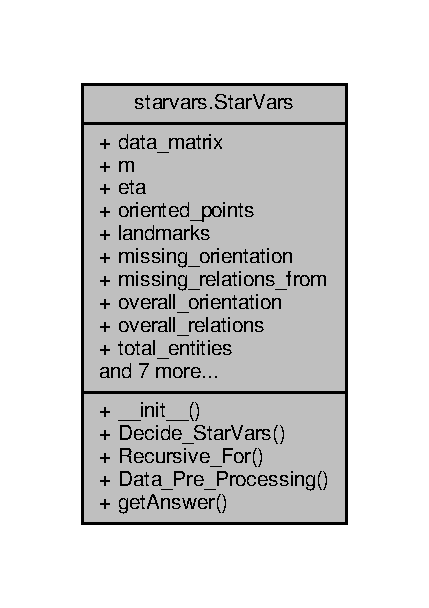
\includegraphics[width=206pt]{classstarvars_1_1StarVars__coll__graph}
\end{center}
\end{figure}
\subsection*{Public Member Functions}
\begin{DoxyCompactItemize}
\item 
def \hyperlink{classstarvars_1_1StarVars_a3394a0e46a1f5cb173821af6fbab07b7}{\-\_\-\-\_\-init\-\_\-\-\_\-}
\item 
def \hyperlink{classstarvars_1_1StarVars_af4960326446ecb6a19a5ae4809516a7f}{Decide\-\_\-\-Star\-Vars}
\item 
def \hyperlink{classstarvars_1_1StarVars_ad9148407d0cb17d568776803518cc611}{Recursive\-\_\-\-For}
\item 
def \hyperlink{classstarvars_1_1StarVars_adadc98f75e2ac694fc13fff32300c60f}{Data\-\_\-\-Pre\-\_\-\-Processing}
\item 
def \hyperlink{classstarvars_1_1StarVars_a28f4018d592ba55987d7e6a4d5bdf8e2}{get\-Answer}
\end{DoxyCompactItemize}
\subsection*{Public Attributes}
\begin{DoxyCompactItemize}
\item 
\hyperlink{classstarvars_1_1StarVars_a0deb0b64b74ef8f10a7941f042741db4}{data\-\_\-matrix}
\item 
\hyperlink{classstarvars_1_1StarVars_acb182bf64bd4d1786654881f758a3285}{m}
\item 
\hyperlink{classstarvars_1_1StarVars_a6ea108f66bbd8f5744dc15dac70905a7}{eta}
\item 
\hyperlink{classstarvars_1_1StarVars_a7dcf860cb0c4d7cd67a0e4078656a286}{oriented\-\_\-points}
\item 
\hyperlink{classstarvars_1_1StarVars_a8e56638a942f24a9929b50ad895db412}{landmarks}
\item 
\hyperlink{classstarvars_1_1StarVars_a1e0d57adb59ce8bb33bd892d96c9b2f6}{missing\-\_\-orientation}
\item 
\hyperlink{classstarvars_1_1StarVars_ad5acc05763dcb07361ad63adb12ea80c}{missing\-\_\-relations\-\_\-from}
\item 
\hyperlink{classstarvars_1_1StarVars_a151e74e8625e7887bc53a6436e09a958}{overall\-\_\-orientation}
\item 
\hyperlink{classstarvars_1_1StarVars_ad332c549295c22b5b86e820253a7125a}{overall\-\_\-relations}
\item 
\hyperlink{classstarvars_1_1StarVars_ae422b5451a6755af3cbd275608756ed1}{total\-\_\-entities}
\item 
\hyperlink{classstarvars_1_1StarVars_ac65a61b0589e992831bc31185ca1cae7}{loopnum}
\item 
\hyperlink{classstarvars_1_1StarVars_a49126602e2b9e3b37bf3935ec387997c}{variable\-\_\-list}
\item 
\hyperlink{classstarvars_1_1StarVars_a5ef4b1343fefb0ec498a456b12d741e1}{orient\-\_\-index}
\item 
\hyperlink{classstarvars_1_1StarVars_a228e7e86033c3b18aa6713a71cb17077}{relations\-\_\-index}
\item 
\hyperlink{classstarvars_1_1StarVars_ac079b3194d890372bc64d1d6feb76874}{xy\-\_\-answer}
\item 
\hyperlink{classstarvars_1_1StarVars_a33ced1c7a9724fe809f86dd06251f023}{overall\-\_\-orientation\-\_\-answer}
\item 
\hyperlink{classstarvars_1_1StarVars_a36974111eb721cc769fb513cfe1db089}{overall\-\_\-relations\-\_\-answer}
\end{DoxyCompactItemize}


\subsection{Detailed Description}
\begin{DoxyVerb}StarVars class teste \end{DoxyVerb}
 

\subsection{Constructor \& Destructor Documentation}
\hypertarget{classstarvars_1_1StarVars_a3394a0e46a1f5cb173821af6fbab07b7}{\index{starvars\-::\-Star\-Vars@{starvars\-::\-Star\-Vars}!\-\_\-\-\_\-init\-\_\-\-\_\-@{\-\_\-\-\_\-init\-\_\-\-\_\-}}
\index{\-\_\-\-\_\-init\-\_\-\-\_\-@{\-\_\-\-\_\-init\-\_\-\-\_\-}!starvars::StarVars@{starvars\-::\-Star\-Vars}}
\subsubsection[{\-\_\-\-\_\-init\-\_\-\-\_\-}]{\setlength{\rightskip}{0pt plus 5cm}def starvars.\-Star\-Vars.\-\_\-\-\_\-init\-\_\-\-\_\- (
\begin{DoxyParamCaption}
\item[{}]{self}
\end{DoxyParamCaption}
)}}\label{classstarvars_1_1StarVars_a3394a0e46a1f5cb173821af6fbab07b7}


\subsection{Member Function Documentation}
\hypertarget{classstarvars_1_1StarVars_adadc98f75e2ac694fc13fff32300c60f}{\index{starvars\-::\-Star\-Vars@{starvars\-::\-Star\-Vars}!Data\-\_\-\-Pre\-\_\-\-Processing@{Data\-\_\-\-Pre\-\_\-\-Processing}}
\index{Data\-\_\-\-Pre\-\_\-\-Processing@{Data\-\_\-\-Pre\-\_\-\-Processing}!starvars::StarVars@{starvars\-::\-Star\-Vars}}
\subsubsection[{Data\-\_\-\-Pre\-\_\-\-Processing}]{\setlength{\rightskip}{0pt plus 5cm}def starvars.\-Star\-Vars.\-Data\-\_\-\-Pre\-\_\-\-Processing (
\begin{DoxyParamCaption}
\item[{}]{self}
\end{DoxyParamCaption}
)}}\label{classstarvars_1_1StarVars_adadc98f75e2ac694fc13fff32300c60f}
\hypertarget{classstarvars_1_1StarVars_af4960326446ecb6a19a5ae4809516a7f}{\index{starvars\-::\-Star\-Vars@{starvars\-::\-Star\-Vars}!Decide\-\_\-\-Star\-Vars@{Decide\-\_\-\-Star\-Vars}}
\index{Decide\-\_\-\-Star\-Vars@{Decide\-\_\-\-Star\-Vars}!starvars::StarVars@{starvars\-::\-Star\-Vars}}
\subsubsection[{Decide\-\_\-\-Star\-Vars}]{\setlength{\rightskip}{0pt plus 5cm}def starvars.\-Star\-Vars.\-Decide\-\_\-\-Star\-Vars (
\begin{DoxyParamCaption}
\item[{}]{self, }
\item[{}]{variable\-\_\-list}
\end{DoxyParamCaption}
)}}\label{classstarvars_1_1StarVars_af4960326446ecb6a19a5ae4809516a7f}


Here is the caller graph for this function\-:\nopagebreak
\begin{figure}[H]
\begin{center}
\leavevmode
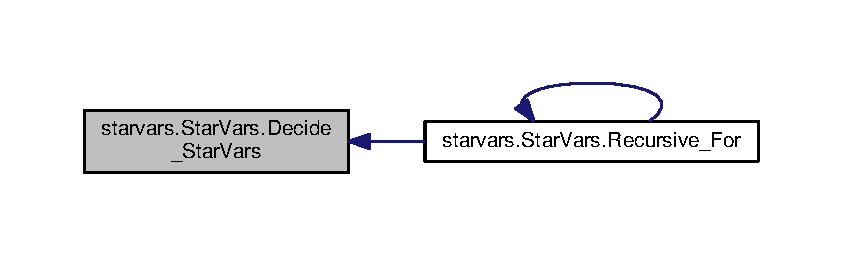
\includegraphics[width=350pt]{classstarvars_1_1StarVars_af4960326446ecb6a19a5ae4809516a7f_icgraph}
\end{center}
\end{figure}


\hypertarget{classstarvars_1_1StarVars_a28f4018d592ba55987d7e6a4d5bdf8e2}{\index{starvars\-::\-Star\-Vars@{starvars\-::\-Star\-Vars}!get\-Answer@{get\-Answer}}
\index{get\-Answer@{get\-Answer}!starvars::StarVars@{starvars\-::\-Star\-Vars}}
\subsubsection[{get\-Answer}]{\setlength{\rightskip}{0pt plus 5cm}def starvars.\-Star\-Vars.\-get\-Answer (
\begin{DoxyParamCaption}
\item[{}]{self}
\end{DoxyParamCaption}
)}}\label{classstarvars_1_1StarVars_a28f4018d592ba55987d7e6a4d5bdf8e2}
\hypertarget{classstarvars_1_1StarVars_ad9148407d0cb17d568776803518cc611}{\index{starvars\-::\-Star\-Vars@{starvars\-::\-Star\-Vars}!Recursive\-\_\-\-For@{Recursive\-\_\-\-For}}
\index{Recursive\-\_\-\-For@{Recursive\-\_\-\-For}!starvars::StarVars@{starvars\-::\-Star\-Vars}}
\subsubsection[{Recursive\-\_\-\-For}]{\setlength{\rightskip}{0pt plus 5cm}def starvars.\-Star\-Vars.\-Recursive\-\_\-\-For (
\begin{DoxyParamCaption}
\item[{}]{self, }
\item[{}]{variable\-\_\-list, }
\item[{}]{n}
\end{DoxyParamCaption}
)}}\label{classstarvars_1_1StarVars_ad9148407d0cb17d568776803518cc611}


Here is the call graph for this function\-:\nopagebreak
\begin{figure}[H]
\begin{center}
\leavevmode
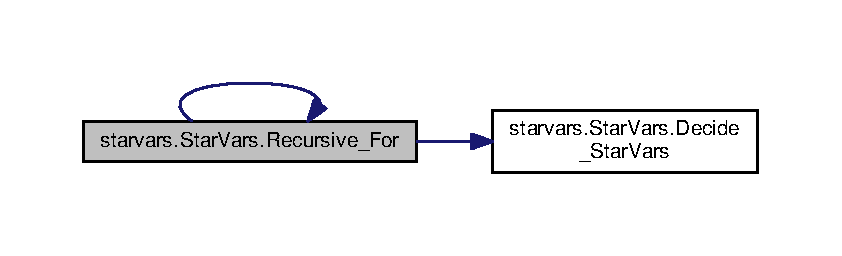
\includegraphics[width=350pt]{classstarvars_1_1StarVars_ad9148407d0cb17d568776803518cc611_cgraph}
\end{center}
\end{figure}




Here is the caller graph for this function\-:\nopagebreak
\begin{figure}[H]
\begin{center}
\leavevmode
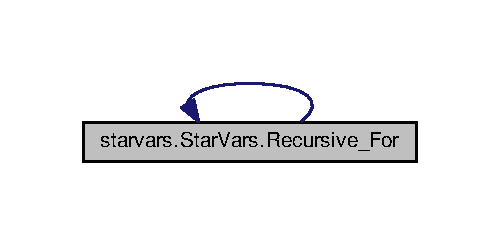
\includegraphics[width=240pt]{classstarvars_1_1StarVars_ad9148407d0cb17d568776803518cc611_icgraph}
\end{center}
\end{figure}




\subsection{Member Data Documentation}
\hypertarget{classstarvars_1_1StarVars_a0deb0b64b74ef8f10a7941f042741db4}{\index{starvars\-::\-Star\-Vars@{starvars\-::\-Star\-Vars}!data\-\_\-matrix@{data\-\_\-matrix}}
\index{data\-\_\-matrix@{data\-\_\-matrix}!starvars::StarVars@{starvars\-::\-Star\-Vars}}
\subsubsection[{data\-\_\-matrix}]{\setlength{\rightskip}{0pt plus 5cm}starvars.\-Star\-Vars.\-data\-\_\-matrix}}\label{classstarvars_1_1StarVars_a0deb0b64b74ef8f10a7941f042741db4}


data matrix teste 

spliting received string

converting data to numpy matrix \hypertarget{classstarvars_1_1StarVars_a6ea108f66bbd8f5744dc15dac70905a7}{\index{starvars\-::\-Star\-Vars@{starvars\-::\-Star\-Vars}!eta@{eta}}
\index{eta@{eta}!starvars::StarVars@{starvars\-::\-Star\-Vars}}
\subsubsection[{eta}]{\setlength{\rightskip}{0pt plus 5cm}starvars.\-Star\-Vars.\-eta}}\label{classstarvars_1_1StarVars_a6ea108f66bbd8f5744dc15dac70905a7}


regions in degrees 

\hypertarget{classstarvars_1_1StarVars_a8e56638a942f24a9929b50ad895db412}{\index{starvars\-::\-Star\-Vars@{starvars\-::\-Star\-Vars}!landmarks@{landmarks}}
\index{landmarks@{landmarks}!starvars::StarVars@{starvars\-::\-Star\-Vars}}
\subsubsection[{landmarks}]{\setlength{\rightskip}{0pt plus 5cm}starvars.\-Star\-Vars.\-landmarks}}\label{classstarvars_1_1StarVars_a8e56638a942f24a9929b50ad895db412}


get landmarks \#\#\# 

\hypertarget{classstarvars_1_1StarVars_ac65a61b0589e992831bc31185ca1cae7}{\index{starvars\-::\-Star\-Vars@{starvars\-::\-Star\-Vars}!loopnum@{loopnum}}
\index{loopnum@{loopnum}!starvars::StarVars@{starvars\-::\-Star\-Vars}}
\subsubsection[{loopnum}]{\setlength{\rightskip}{0pt plus 5cm}starvars.\-Star\-Vars.\-loopnum}}\label{classstarvars_1_1StarVars_ac65a61b0589e992831bc31185ca1cae7}
\hypertarget{classstarvars_1_1StarVars_acb182bf64bd4d1786654881f758a3285}{\index{starvars\-::\-Star\-Vars@{starvars\-::\-Star\-Vars}!m@{m}}
\index{m@{m}!starvars::StarVars@{starvars\-::\-Star\-Vars}}
\subsubsection[{m}]{\setlength{\rightskip}{0pt plus 5cm}starvars.\-Star\-Vars.\-m}}\label{classstarvars_1_1StarVars_acb182bf64bd4d1786654881f758a3285}


granularity 

\hypertarget{classstarvars_1_1StarVars_a1e0d57adb59ce8bb33bd892d96c9b2f6}{\index{starvars\-::\-Star\-Vars@{starvars\-::\-Star\-Vars}!missing\-\_\-orientation@{missing\-\_\-orientation}}
\index{missing\-\_\-orientation@{missing\-\_\-orientation}!starvars::StarVars@{starvars\-::\-Star\-Vars}}
\subsubsection[{missing\-\_\-orientation}]{\setlength{\rightskip}{0pt plus 5cm}starvars.\-Star\-Vars.\-missing\-\_\-orientation}}\label{classstarvars_1_1StarVars_a1e0d57adb59ce8bb33bd892d96c9b2f6}


get missing orientations \#\#\# 

\hypertarget{classstarvars_1_1StarVars_ad5acc05763dcb07361ad63adb12ea80c}{\index{starvars\-::\-Star\-Vars@{starvars\-::\-Star\-Vars}!missing\-\_\-relations\-\_\-from@{missing\-\_\-relations\-\_\-from}}
\index{missing\-\_\-relations\-\_\-from@{missing\-\_\-relations\-\_\-from}!starvars::StarVars@{starvars\-::\-Star\-Vars}}
\subsubsection[{missing\-\_\-relations\-\_\-from}]{\setlength{\rightskip}{0pt plus 5cm}starvars.\-Star\-Vars.\-missing\-\_\-relations\-\_\-from}}\label{classstarvars_1_1StarVars_ad5acc05763dcb07361ad63adb12ea80c}


get missing relations \#\#\# 

\hypertarget{classstarvars_1_1StarVars_a5ef4b1343fefb0ec498a456b12d741e1}{\index{starvars\-::\-Star\-Vars@{starvars\-::\-Star\-Vars}!orient\-\_\-index@{orient\-\_\-index}}
\index{orient\-\_\-index@{orient\-\_\-index}!starvars::StarVars@{starvars\-::\-Star\-Vars}}
\subsubsection[{orient\-\_\-index}]{\setlength{\rightskip}{0pt plus 5cm}starvars.\-Star\-Vars.\-orient\-\_\-index}}\label{classstarvars_1_1StarVars_a5ef4b1343fefb0ec498a456b12d741e1}
\hypertarget{classstarvars_1_1StarVars_a7dcf860cb0c4d7cd67a0e4078656a286}{\index{starvars\-::\-Star\-Vars@{starvars\-::\-Star\-Vars}!oriented\-\_\-points@{oriented\-\_\-points}}
\index{oriented\-\_\-points@{oriented\-\_\-points}!starvars::StarVars@{starvars\-::\-Star\-Vars}}
\subsubsection[{oriented\-\_\-points}]{\setlength{\rightskip}{0pt plus 5cm}starvars.\-Star\-Vars.\-oriented\-\_\-points}}\label{classstarvars_1_1StarVars_a7dcf860cb0c4d7cd67a0e4078656a286}


get oriented points \#\#\# 

\hypertarget{classstarvars_1_1StarVars_a151e74e8625e7887bc53a6436e09a958}{\index{starvars\-::\-Star\-Vars@{starvars\-::\-Star\-Vars}!overall\-\_\-orientation@{overall\-\_\-orientation}}
\index{overall\-\_\-orientation@{overall\-\_\-orientation}!starvars::StarVars@{starvars\-::\-Star\-Vars}}
\subsubsection[{overall\-\_\-orientation}]{\setlength{\rightskip}{0pt plus 5cm}starvars.\-Star\-Vars.\-overall\-\_\-orientation}}\label{classstarvars_1_1StarVars_a151e74e8625e7887bc53a6436e09a958}
\hypertarget{classstarvars_1_1StarVars_a33ced1c7a9724fe809f86dd06251f023}{\index{starvars\-::\-Star\-Vars@{starvars\-::\-Star\-Vars}!overall\-\_\-orientation\-\_\-answer@{overall\-\_\-orientation\-\_\-answer}}
\index{overall\-\_\-orientation\-\_\-answer@{overall\-\_\-orientation\-\_\-answer}!starvars::StarVars@{starvars\-::\-Star\-Vars}}
\subsubsection[{overall\-\_\-orientation\-\_\-answer}]{\setlength{\rightskip}{0pt plus 5cm}starvars.\-Star\-Vars.\-overall\-\_\-orientation\-\_\-answer}}\label{classstarvars_1_1StarVars_a33ced1c7a9724fe809f86dd06251f023}
\hypertarget{classstarvars_1_1StarVars_ad332c549295c22b5b86e820253a7125a}{\index{starvars\-::\-Star\-Vars@{starvars\-::\-Star\-Vars}!overall\-\_\-relations@{overall\-\_\-relations}}
\index{overall\-\_\-relations@{overall\-\_\-relations}!starvars::StarVars@{starvars\-::\-Star\-Vars}}
\subsubsection[{overall\-\_\-relations}]{\setlength{\rightskip}{0pt plus 5cm}starvars.\-Star\-Vars.\-overall\-\_\-relations}}\label{classstarvars_1_1StarVars_ad332c549295c22b5b86e820253a7125a}
\hypertarget{classstarvars_1_1StarVars_a36974111eb721cc769fb513cfe1db089}{\index{starvars\-::\-Star\-Vars@{starvars\-::\-Star\-Vars}!overall\-\_\-relations\-\_\-answer@{overall\-\_\-relations\-\_\-answer}}
\index{overall\-\_\-relations\-\_\-answer@{overall\-\_\-relations\-\_\-answer}!starvars::StarVars@{starvars\-::\-Star\-Vars}}
\subsubsection[{overall\-\_\-relations\-\_\-answer}]{\setlength{\rightskip}{0pt plus 5cm}starvars.\-Star\-Vars.\-overall\-\_\-relations\-\_\-answer}}\label{classstarvars_1_1StarVars_a36974111eb721cc769fb513cfe1db089}
\hypertarget{classstarvars_1_1StarVars_a228e7e86033c3b18aa6713a71cb17077}{\index{starvars\-::\-Star\-Vars@{starvars\-::\-Star\-Vars}!relations\-\_\-index@{relations\-\_\-index}}
\index{relations\-\_\-index@{relations\-\_\-index}!starvars::StarVars@{starvars\-::\-Star\-Vars}}
\subsubsection[{relations\-\_\-index}]{\setlength{\rightskip}{0pt plus 5cm}starvars.\-Star\-Vars.\-relations\-\_\-index}}\label{classstarvars_1_1StarVars_a228e7e86033c3b18aa6713a71cb17077}
\hypertarget{classstarvars_1_1StarVars_ae422b5451a6755af3cbd275608756ed1}{\index{starvars\-::\-Star\-Vars@{starvars\-::\-Star\-Vars}!total\-\_\-entities@{total\-\_\-entities}}
\index{total\-\_\-entities@{total\-\_\-entities}!starvars::StarVars@{starvars\-::\-Star\-Vars}}
\subsubsection[{total\-\_\-entities}]{\setlength{\rightskip}{0pt plus 5cm}starvars.\-Star\-Vars.\-total\-\_\-entities}}\label{classstarvars_1_1StarVars_ae422b5451a6755af3cbd275608756ed1}
\hypertarget{classstarvars_1_1StarVars_a49126602e2b9e3b37bf3935ec387997c}{\index{starvars\-::\-Star\-Vars@{starvars\-::\-Star\-Vars}!variable\-\_\-list@{variable\-\_\-list}}
\index{variable\-\_\-list@{variable\-\_\-list}!starvars::StarVars@{starvars\-::\-Star\-Vars}}
\subsubsection[{variable\-\_\-list}]{\setlength{\rightskip}{0pt plus 5cm}starvars.\-Star\-Vars.\-variable\-\_\-list}}\label{classstarvars_1_1StarVars_a49126602e2b9e3b37bf3935ec387997c}
\hypertarget{classstarvars_1_1StarVars_ac079b3194d890372bc64d1d6feb76874}{\index{starvars\-::\-Star\-Vars@{starvars\-::\-Star\-Vars}!xy\-\_\-answer@{xy\-\_\-answer}}
\index{xy\-\_\-answer@{xy\-\_\-answer}!starvars::StarVars@{starvars\-::\-Star\-Vars}}
\subsubsection[{xy\-\_\-answer}]{\setlength{\rightskip}{0pt plus 5cm}starvars.\-Star\-Vars.\-xy\-\_\-answer}}\label{classstarvars_1_1StarVars_ac079b3194d890372bc64d1d6feb76874}


The documentation for this class was generated from the following file\-:\begin{DoxyCompactItemize}
\item 
\hyperlink{starvars_8py}{starvars.\-py}\end{DoxyCompactItemize}

\chapter{File Documentation}
\hypertarget{main_8py}{\section{main.\-py File Reference}
\label{main_8py}\index{main.\-py@{main.\-py}}
}
\subsection*{Namespaces}
\begin{DoxyCompactItemize}
\item 
\hyperlink{namespacemain}{main}
\end{DoxyCompactItemize}
\subsection*{Functions}
\begin{DoxyCompactItemize}
\item 
def \hyperlink{namespacemain_a021bfca46dd0435fb213d09cf10db27e}{main.\-main}
\end{DoxyCompactItemize}
\subsection*{Variables}
\begin{DoxyCompactItemize}
\item 
string \hyperlink{namespacemain_a5e2661c5c42dc197ee8e68887453d3bc}{main.\-\_\-\-\_\-author\-\_\-\-\_\-} = \char`\"{}Danilo H. Perico\char`\"{}
\item 
string \hyperlink{namespacemain_a70420639202607ff61f0a08061e04e47}{main.\-\_\-\-\_\-license\-\_\-\-\_\-} = \char`\"{}G\-N\-U General Public License v3.\-0\char`\"{}
\item 
string \hyperlink{namespacemain_afb7b6dcaed6631460aa4089c3b178748}{main.\-\_\-\-\_\-project\-\_\-\-\_\-} = \char`\"{}Probabilistic Star\-Vars\char`\"{}
\end{DoxyCompactItemize}

\hypertarget{oriented__point_8py}{\section{oriented\-\_\-point.\-py File Reference}
\label{oriented__point_8py}\index{oriented\-\_\-point.\-py@{oriented\-\_\-point.\-py}}
}
\subsection*{Classes}
\begin{DoxyCompactItemize}
\item 
class \hyperlink{classoriented__point_1_1OrientedPoint}{oriented\-\_\-point.\-Oriented\-Point}
\end{DoxyCompactItemize}
\subsection*{Namespaces}
\begin{DoxyCompactItemize}
\item 
\hyperlink{namespaceoriented__point}{oriented\-\_\-point}
\end{DoxyCompactItemize}
\subsection*{Variables}
\begin{DoxyCompactItemize}
\item 
string \hyperlink{namespaceoriented__point_aa3b4d2d674d85c3cbe62dd838254d6d0}{oriented\-\_\-point.\-\_\-\-\_\-author\-\_\-\-\_\-} = \char`\"{}Danilo H. Perico\char`\"{}
\item 
string \hyperlink{namespaceoriented__point_a3d6cc46d63eaa6bbf92eff2835e6a1c2}{oriented\-\_\-point.\-\_\-\-\_\-license\-\_\-\-\_\-} = \char`\"{}G\-N\-U General Public License v3.\-0\char`\"{}
\item 
string \hyperlink{namespaceoriented__point_a9691eace975baee6e55c7185dc3bb251}{oriented\-\_\-point.\-\_\-\-\_\-project\-\_\-\-\_\-} = \char`\"{}Probabilistic Star\-Vars\char`\"{}
\end{DoxyCompactItemize}

\hypertarget{starvars_8py}{\section{starvars.\-py File Reference}
\label{starvars_8py}\index{starvars.\-py@{starvars.\-py}}
}
\subsection*{Classes}
\begin{DoxyCompactItemize}
\item 
class \hyperlink{classstarvars_1_1StarVars}{starvars.\-Star\-Vars}
\end{DoxyCompactItemize}
\subsection*{Namespaces}
\begin{DoxyCompactItemize}
\item 
\hyperlink{namespacestarvars}{starvars}
\end{DoxyCompactItemize}
\subsection*{Variables}
\begin{DoxyCompactItemize}
\item 
string \hyperlink{namespacestarvars_ac644d7f280f95cccc18a5d57a812e131}{starvars.\-\_\-\-\_\-author\-\_\-\-\_\-} = \char`\"{}Danilo H. Perico\char`\"{}
\item 
string \hyperlink{namespacestarvars_a1264921cafa3bfaea6a08a307416bbc6}{starvars.\-\_\-\-\_\-license\-\_\-\-\_\-} = \char`\"{}G\-N\-U General Public License v3.\-0\char`\"{}
\item 
string \hyperlink{namespacestarvars_afabb4c7baf270d344e2640778b38e5ff}{starvars.\-\_\-\-\_\-project\-\_\-\-\_\-} = \char`\"{}Probabilistic Star\-Vars\char`\"{}
\end{DoxyCompactItemize}

%--- End generated contents ---

% Index
\newpage
\phantomsection
\addcontentsline{toc}{chapter}{Index}
\printindex

\end{document}
